\documentclass[11pt]{article}
\title{Meccano hexagons gallery}
\author{https://github.com/heptagons/meccano/hexa/gallery}
\date{2023/12/20}

\usepackage{../../meccano}
\usepackage{amssymb}

\begin{document}

\maketitle
\begin{abstract}
We build rigid meccano\meccanoref regular pentagons from sides $4$ to $24$. We restrict all internal strips to remain inside the hexagons's perimeter and don't permit they overlap with others. The internal strips must not be parallel to any side of the hexagon.
\end{abstract}

% 13

\section{Internal strips}

\begin{figure}[h]
\centering
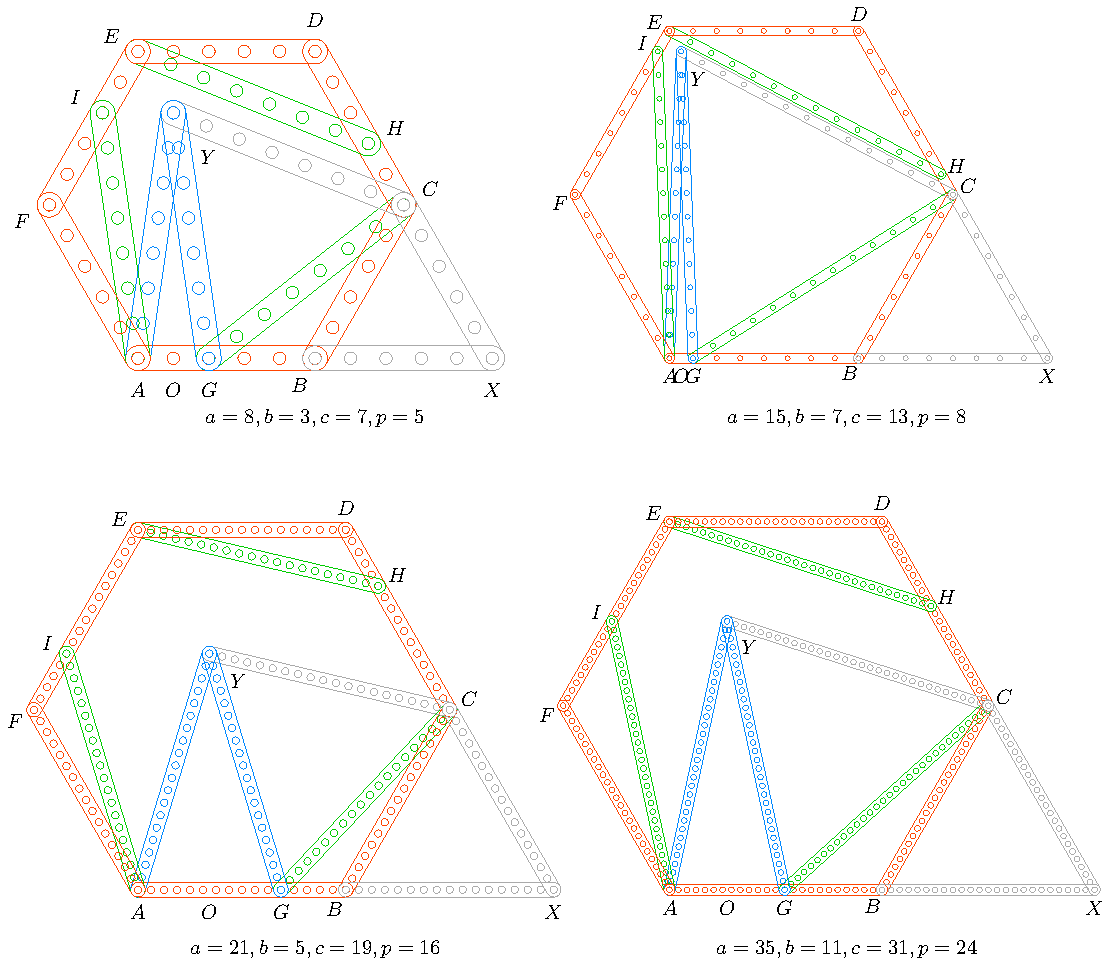
\includegraphics[scale=0.9]{build/hexa-builder-a}
\caption{First four cases where internal strip $c = \overline{GC}$ is an integer and makes rigid two consecutive regular hexagon sides $s = \overline{AB} = \overline{BC}$. We use two numbers to identify every solution $a$ and $b$ where $b = \overline{GB}$ and $a = s - b$ and $c = \sqrt{a^2+b^2-ab}$. }
\label{fig:builder-a}
\end{figure}

We run a software program to look strips that can make rigid two consecutive internal sides of any hexagon. Figure \ref{fig:builder-a} show the smaller four cases found. Consider the figure at top left, the internal hexagon angle is $\theta \equiv \angle{GBC} = 2\pi/3$ and the hexagon side is $s \equiv \overline{BC}$. Consider the triangle $\triangle{GBC}$ and define the other two sides as $b \equiv \overline{GB}$ and $c = \overline{GC}$. By the law of cosines we know that:
\begin{align}
c &= \sqrt{b^2 + s^2 - 2bs\cos\theta} \nonumber\\
 &= \sqrt{b^2 + s^2 - 2bs\left(-\frac{1}{2}\right)} \nonumber\\
 &= \sqrt{b^2 + s^2 + bs}
\end{align}
By defining $a \equiv s + b$ we get:
\begin{align}
c &= \sqrt{a^2 + b^2 - ab} \quad \texttt{ where } a > b
\end{align}
Running the software iterating first over $a$ and then by $b$ and filtering $c$ to be integer we get the first rows:
\begin{center}
\begin{tabular}{||c c c c||} 
 \hline
 $a$ & $b$ & $c$ & $s$ \\ [0.5ex] 
 \hline\hline
  8 &  3 &  7 &  5 \\ \hline
 15 &  7 & 13 &  8 \\ \hline
 21 &  5 & 19 & 16 \\ \hline
 35 & 11 & 31 & 24 \\ \hline
 40 &  7 & 37 & 33 \\ \hline
 48 & 13 & 43 & 35 \\ [1ex] 
 \hline
\end{tabular}
\end{center}

Figure $\ref{fig:builder-a}$ shows hexagons of sizes $s=5,8,16,24$ with perimeter strips in orange can be made rigid adding three internal green strips of lenght $c = 7,13,19,31$. In each case we have an equilateral triangle $\triangle{GCY}$ and an isoscelles triangle $\triangle{AGY}$. The base of the isoscelles triangle is $x \equiv \overline{AG} = \overline{AB} - \overline{GB} = s - b$ and the equals sides $\overline{AY} = \overline{GY} = c$. So we can calculate the height $y \equiv \overline{OY}$:
\begin{align}
y &= \sqrt{(\overline{GY})^2 - (\overline{AO})^2} \nonumber\\
 &= \sqrt{c^2 - \left(\frac{s-b}2\right)^2} \nonumber\\
 &= \sqrt{b^2 + s^2 + bs - \left(\frac{s-b}2\right)^2} = \frac{(b+s)\sqrt3}2 = \frac{a\sqrt3}2
\end{align}

\begin{figure}[h]
\centering
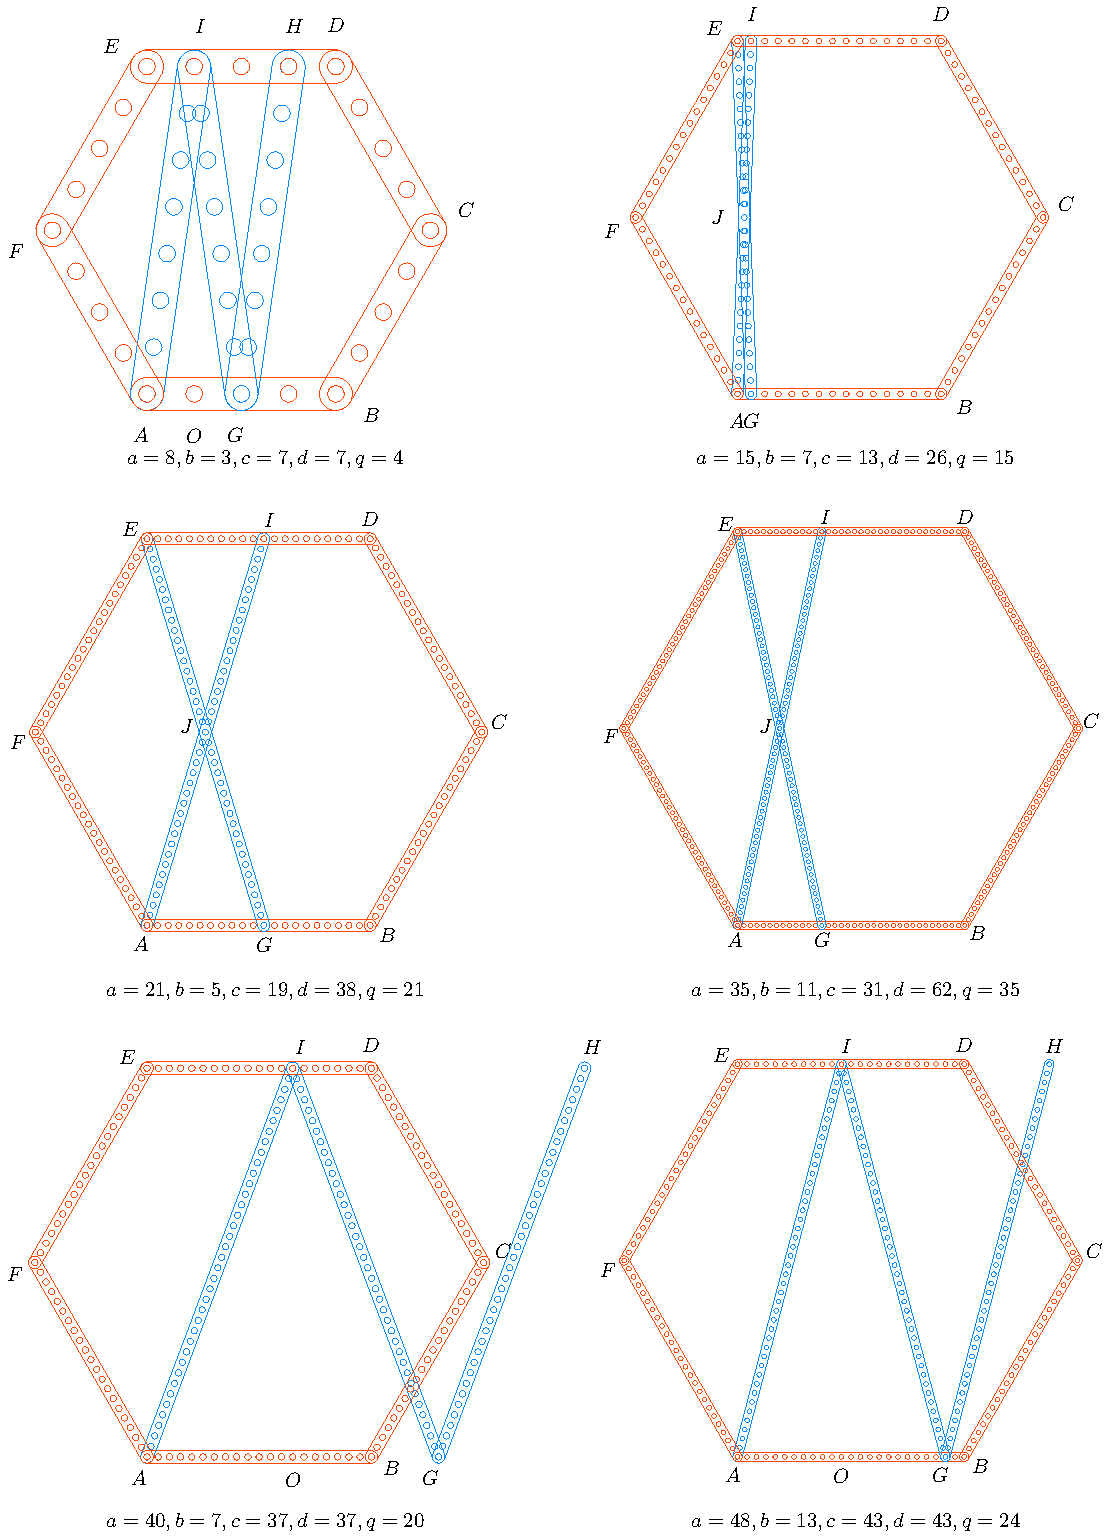
\includegraphics[scale=0.8]{build/hexa-builder-b}
\caption{First six cases of integral distances $c$. When the distance $s-b = \overline{AG}$ is even, we use the strips $d = c$ to join opposites sides of hexagons of side $t = a/2$. When is odd, we use the strips $d = 2c$ to join opposites sides of hexagons of side $t = a$.}
\label{fig:builder-b}
\end{figure}

We know $\frac{a\sqrt3}2$ is the height of the regular hexagon of side $a/2$ so we can use the blue strips to connect opposite sides. Figure \ref{fig:builder-b} show the smaller hexagons that have integer strips connecting opposites sides.

Through the gallery we use the green strips and blue strips and scaled copies to make rigid hexagons from size $4$ to $24$. We prioritize minimum number of bolts, minimum number of strips and the largest strips sizes as possible.

\section{Hexagons of size 13}

\begin{figure}[H]
\centering
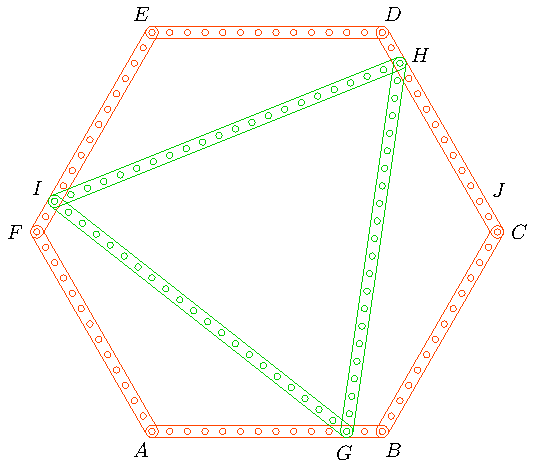
\includegraphics[scale=1]{13/hexa-13a}
\caption{Hexagon of size $s = 13$. Diagonals $c = \overline{GH} = \overline{HI} = \overline{IG} = 21$.}
\label{fig:13a}
\end{figure}

Figure \ref{fig:13a} show hexagon of size $13$. We have an offset of $f = \overline{CJ} = \overline{HD} = 2$ so $\overline{GJ} = \overline{BC} + \overline{CJ} = 13+2 = 15$ and $\overline{JH} = \overline{CD} - 2\overline{CJ} = 13 - 2(2) = 9$.

\end{document}
